\chapter{The LHC and CMS Machine}
In this chapter, the working and the design parameters of L\acrfull{lhc} and its one of main purpose dectector, Compact Muon Solenoid (CMS), is briefly described.

\section{The Large Hadron Collider}
The famous quote ``history repeats itself" applies well to the \acrfull{hep} experiments. The starting point of experimental particle physics is the Rutherford $\alpha$-particle scattering, and even now we are doing the same thing just the method changed from ``natural accelerator" to the ``man-made" accelerator that can accelerate particles with the velocity close to the speed of light. The design and working of accelerator changed a lot over a period of time in going from MeV to GeV and in the TeV range. Now, these machines are not only used in \acrshort{hep} experiments, but extends its arena to treat human beings like cancer therapy, radioisotope production, 3-D x-ray\todo[fancyline]{Add citations to the applications}, also to the industry for uses like material processing, sterilisation, security scan, water treatment, and many more. 

The \acrshort{lhc} is  a hadron collider which can accelerate the two proton beams in opposite direction with maximum of 14 TeV energy in a 26.6 km long tunnel which is about 100 m underground. The \acrshort{lhc} is the latest and most-\todo[fancyline]{Find better word}powerful accelerator everbuilt. It is a proton-proton collider built to improve our understanding of fundamental physics. It started on 21$^{st}$ October 2008. It is built in the same tunnel where there was Large Electron Positron (LEP) collider, that collides electrons and positrons. LEP collaboration decided to switch to hadron collider because of following advantages:
\begin{itemize}
    \item Hadron collider can reach a higher centre of mass (COM) energy, because of much lower synchrotron radiation emitted by hadrons as compared to electrons. Synchrotron radiation loss is directory proportional to $(Energy/mass)^4$. \todo[fancyline]{Add exact number for electrons and protons synchtron loss.}
    \item As hadrons are composit particles so it allows us to scan over wide range of energy.
\end{itemize}


For any particle accelerator there are mainly three components so for the LHC. They are:
\begin{itemize}
  \item Beam pipes
  \item Accelerating structure
  \item Magnet system
\end{itemize}

\subsection{Beam Pipes}
At LHC there are two beam pipes. For each the diameter is $\approx$6.3 cm in which protron beam travels in opposite direction. We should keep the beam pipes with ultra-high vacuum\footnote{At LHC there are three different vacuum systems used. First one is used for beam pipe another is used for insulating the cryogenically cooled magnets and third one is used for insulating the helium distribution. In the later two it it just acts as a thermal insulator as the cryogenic parts are kept at 1.9 K ($\ang{-271.3}C$)} to minimize the number of collision with the gas molecules which result in beam unstability and loss of beam particles. At LHC the beam pipes are kept at $1.013 \times 10^{-13}$ bar pressure.

\subsection{Accelerating Structure}

Another main part of any particle accelerator is its accelerating structure. A accelerator in TeV range can not start from rest and go to the TeV range in one go it should go into several stages depending on the energy. At LHC the jouney of proton starts from grabing the proton from Hydrogen gas and subsequently go into 5 different stages. The stages can be dcreased but could not be just one stage. Here, at accelerating structure also serves several other experiments like ISOLDE, NA, AD,\todo[fancyline]{Add reference to these experiments} and others. Various experiments at LHC accelerating structure are summarized in fig. \ref{fig:OtherExpAtAccStructure}.
\begin{figure}[h]
  \begin{center}
  \includegraphics[scale=0.5]{figures/LHC/distribution_of_protons_en.jpg}
  \caption{Other experiments at the LHC accelerating chain \cite{OtherExpAtLHCAcceleratingChain}}
  \label{fig:OtherExpAtAccStructure}
  \end{center}
\end{figure}
The acceleration of protons are done in several steps. \todo[fancyline]{Write again the accelerator chain information.} They are:
\begin{itemize}
    \item Grab proton source: The source of proton is Duoplasmatron\footnote{It strips electron from hydrogen gas and creates a plasma of protons, electrons and molecular ions. This plasma expands towards the extraction electrodes and a protom beam is formed}\cite{LHC-tdr-vol3}. This feed protons to LINAC2.
    \item LINAC2 (Linear accelerator-2): It is the starting point of proton's journey in the LHC accelerator complex. Here, protons reaches to an energy of 50 $MeV$ using the radiofrequency (RF) cavities\footnote{A RF cavity is an mettalic cavity that accelerates the charged particles using the electromagnetic field.} where it also gains 5\% in mass. It feeds to the Proton Synchtron Booster (PSB).
    \item PSB: It takes 50 $MeV$ protons beams from LINAC2 and accelerates it to 1.4 $GeV$ for the injection into Proton Synchtron (PS).
    \item PS: It is one of key component in the LHC accelerator complex. It increases the energy of protons upto 25 $GeV$ and feeds to super proton synchtron.
    \item Super Proton Synchtron (SPS): It has a circumference of 7 $km$ where protons are accelerated to an energy of 450 $GeV$. Then via two transmission line protons are then injected into LHC ring.
    \item LHC: It grabs two proton beams from SPS which is injected into opposite direction in parallel pipes. In LHC proton beams can be accelerated upto 7 $TeV$.
\end{itemize}
The CERN accelerator complex is shown in Fig. \ref{fig:CERN-accelerator-complex}.  
\begin{figure}[!ht]
  % \centering
  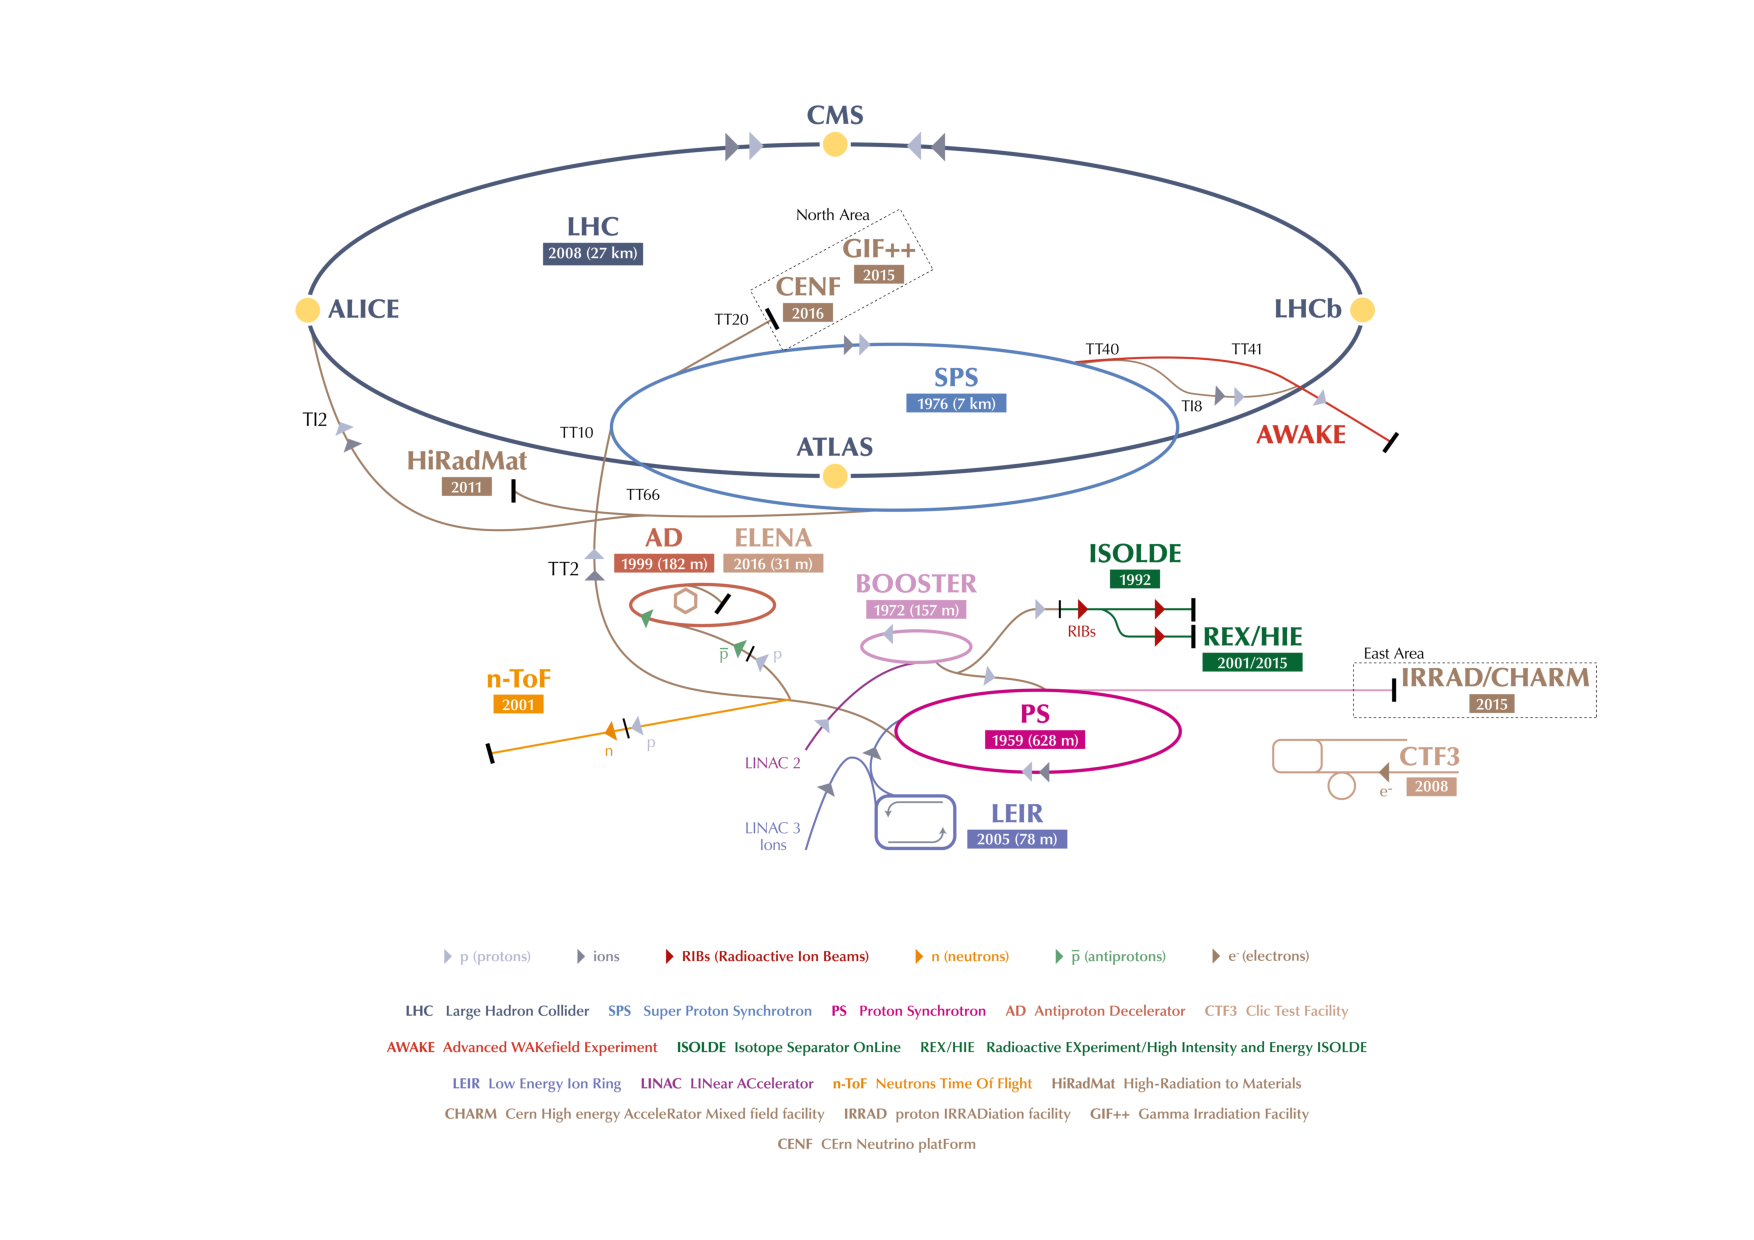
\includegraphics[width=16cm,height=18cm]{figures/CERN_Accelerator_Complex-v2016.pdf}
  \caption{The LHC is the last ring (dark blue line) in a complex chain of particle accelerators. The smaller machines are used in a chain to help boost the particles to their final energies and provide beams to a whole set of smaller experiments, which also aim to uncover the mysteries of the Universe.\todo[inline]{Update the caption.} \cite{Fig-CERN-accelerator-complex}}
  \label{fig:CERN-accelerator-complex}
\end{figure}


\subsection{Magnet System}
As the LHC is a circular collider so magenet system is its one of core part which give them a circular trajectory in the LHC beam pipes. Magnet systems are not just for bending the beam but along with that to focus and for making various corrections we need this\todo[fancyline]{name the corrections.}. To be economical LHC is made in eight arcs and eight straight sections instead of a perfect circle. Along with the bending of beam it is also negessary to focus the beam as the same charge protons try to diverge. To focus the beam a pair of quadrapole magnets are used one focuses the beam width while other foucs the beam height. There are total of 858 quadrupole magnets are installed in LHC to keep the beam focused. Along with this every protons in the beam are not exactly with the same energy and in same path. To correct this focusing with change in energy there are sextupoles magnets are used. There are several other magnetic multipoles are used that help us to keep beam focused if the beam suffers from gravitational interactions over protons, electromagnetic interactions among bunchees, electron clouds from pipe wall, and so on. Different types of magnets used in LHC are listed here \cite{WebLink:LHC_magnets}. Along with this there are eight sets of "inner triplets" are used. These are used at the four interaction points to focus the beam while collide to increase the luminosity. Here the size of bunch goes from 0.2mm to 17 $\mu m$ at the interaction point of ATLAS or CMS. At the interaction point of ALICE or LHCb it is 71 $\mu m$.


Because of limited geometrical space in LHC ring the beam pipe was designed as a ``twin-aperture" magnets, where superconducing ring is housed in a common return yoke and cryostat.


\begin{figure}[h]
  \begin{center}
  \includegraphics[scale=0.8]{figures/LHC/lhc-schematic.jpg}
  \caption{LHC geometry with arcs and straight sections. }
  \label{fig:LHCgeometry}
  \end{center}
\end{figure}


\begin{figure}[h]
  \begin{center}
  \includegraphics[scale=1.0]{figures/LHC/quadrupole_magnet_pair.png}
  \caption{LHC geometry with arcs and straight sections. }
  \label{fig:QuadrupoleMagnet}
  \end{center}
\end{figure}

\section{Other Information to be organized}



The interaction in HEP experiments are characterized mainly by the center of mass energy along with type and number of particles. Summary of important parameters of LHC is given in Table-\ref{table:LHC-parameters}.

\begin{table}
\centering
\begin{tabular}[!ht]{l c}
\hline
{\bf Parameters} & {\bf Value} \\
\hline
Circumference of LHC ring   &   26658.883 m \\
\hline
Maximum dipole magnetic field   & 8.33 T \\
Dipole operating temperature    & 1.9 K \\
\hline
Maximum stored energy per beam (nominal) &   362 MJ \\
Maximum stored energy per beam  (2012) &   143 MJ \\
Maximum stored energy per beam  (2016) &   266 MJ \\
\hline
Beam energy at Injection    & 450 GeV \\
Beam energy at collision (nominal) &    7 TeV \\
Beam energy at collision (2012)     &   4 TeV \\
Beam energy at collision (2016)     &   6.5 TeV \\
\hline
Maximum instantaneous luminosity (nominal)  &   $10^{34}$ cm$^-2$ s$^{-1}$ \\
Maximum instantaneous luminosity (2012)     &   $7.7 \times 10^{33}$ cm$^-2$ s$^{-1}$ \\
Maximum instantaneous luminosity (2016)     &   $1.4 \times 10^{34}$ cm$^-2$ s$^{-1}$ \\
\hline
Number of bunches per proton beam (nominal) &   2808 \\
Number of bunches per proton beam (2012)    &   1380 \\
Number of bunches per proton beam (2016)    &   2076 \\
Maximum number of protons per bunch         &   $1.6 \times 10^{11}$ \\
\hline
Protons/bunch (average at start of collision) (nominal)   &   $1.15 \times 10^{11}$ \\
Protons/bunch (average at start of collision) (2012)  &   $1.5 \times 10^{11}$ \\
Protons/bunch (average at start of collision) (2016)  &   $1.1 \times 10^{11}$ \\
\hline
Bunch collision frequency (nominal)         &   40 MHz  \\
Bunch collision frequency (2012)            &   20 MHz  \\
Bunch collision frequency (2016)            &   40 MHz  \\
\hline
Bunch length (at injection)   &   1.7 ns \\
Bunch length (at collision)   &   1.05 ns \\
Energy spread (at injection)   &   1.9$\times 10^{-3}$ \\
Energy spread (at collision)   &   0.45$\times 10^{-3}$  \\
\hline
Half crossing angle  (nominal)   & 143 $\mu rad$ \\
Half crossing angle  (2012)   & 146 $\mu rad$ \\
Half crossing angle  (2016)   & 185 $\mu rad$ \\
\hline
$\beta *$  (nominal) &   0.55 m\\
$\beta *$   (2012)&   0.6 m\\
$\beta *$   (2016)&   0.4 m\\
\hline
RMS beam size at IP1 \& IP5 &   17 $\mu m$ \\
RMS beam size at IP2 \& IP8 &   71 $\mu m$ \\
\hline
$\epsilon_n$(transverse emittance, rms, normalized) (at injection) &   3.5 $\mu$m\\
$\epsilon_n$(transverse emittance, rms, normalized) (at collision point) &   3.75 $\mu$m\\
\hline
total longitudinal emittance (at injection) & 1.0 eVs \\
total longitudinal emittance (at collision) & 2.5 eVs \\
\hline
Average mean pile-up (nominal) &   \begin{minipage}{5cm} \todo[inline]{Add pile-up for 2012 and 2016}\end{minipage} \\
Average mean pile-up (2012) &    ?? \\
Average mean pile-up (2016) &    ?? \\
\hline
Energy loss per turn at 14 TeV              &   7 keV   \\
Energy loss per turn for electrons          &  \begin{minipage}{5cm}  \todo[inline]{add synchtron energy loss for electrons} \end{minipage}     \\
\end{tabular}
\caption{LHC technical parameters for proton-proton collisions: nominal, 2012 and 2016 values.\cite{Bruce2016, Schoerner-Sadenius2015, LHC-parameters-2016, LHC-tdr-vol1}.}
\label{table:LHC-parameters}
\end{table}




\subsection{LHC Requirements}
For a collider like LHC the figure of merit   

    is luminosity. The luminosity is proportional to the number of events per second so it shold be maximized. Luminosity is defined as:
\begin{equation}
    L = \frac{k_bN_b^2f_{rev}\gamma}{4 \pi \epsilon_n \beta^*}
\end{equation}
where,\\
\hspace{2cm}$k_b$ is the number of bunches per ring,\\
\hspace{2cm}$N_b$ is the number of protons per bunch,\\
\hspace{2cm}$f_{rev}$ the revolution frequency,\\
\hspace{2cm}$\epsilon_n$ is the normalized RMS transverse beam emittance (same in both )\\
\hspace{2cm}$\beta^*$ is the beta-function at the interaction point\\

Based on the definition of luminosity, we can maximize it by following means:
\begin{itemize}
    \item By decreasing beam emittence, $\epsilon_n$.
    \item By improving the cryogenic system. As the factor $k_b.N_b$ is limited by thermal energy produced by synchtron radiation.
    \item By decreasing beam-beam effect\todo[fancyline]{add reference of beam-beam effect}. As it scales with $N_b/ \epsilon_n$ which causees the spread in betatron tunes\todo[fancyline]{add reference of betatron tunes}.
    \item Also, the space charge \todo[fancyline]{add Reference of space-charge} scales with $N_b/ \epsilon_n$.
\end{itemize}



\begin{figure}[!ht]
  % \centering
  \includegraphics[width=12cm,height=10cm]{figures/lumi-proj-2016-final-v2}
  \caption{The integrated luminosity of the LHC with proton-proton collisions in 2016 compared to previous years. Luminosity is a measure of a collider’s efficiency and is proportional to the number of collisions. The integrated luminosity achieved by the LHC in 2016 far surpassed expectations and is double that achieved at a lower energy in 2012. (Image : CERN)\todo[inline]{Update the caption.}} 
  \label{fig:lumi-proj-2016-final-v2}
\end{figure}
